\documentclass[a4paper, 11pt, parskip, colorful]{lecturenotes}

% lualatex -shell-escape -aux-dir=".aux" main.tex

\author{Daniel Jakob}
\makeatletter
\modulecode{MEEN40060}
\modulename{Fracture Mechanics}
\modulecoord{Dr Neal Murphy (\email{neal.murphy@ucd.ie})}
\modulelecturers{Dr Neal Murphy}
\moduletas{Dr Ehsan Rezvani}
\title{\@modulecode~\@modulename~--~Lecture Notes and Module Related Content}
\makeatother

\begin{document}

\pdfbookmark[-1]{Title Page}{titlepage}

\maketitle
\makeatletter

\noindent Coordinator: \@modulecoord \\
Lecturers: \@modulelecturers \\
TAs: \@moduletas
\makeatother

\textbf{Lecture Timetable:}\\
36 lectures, 3 per week during Semester 1
\begin{itemize}
    \item[] Monday 10am Room 216/Zoom
    \item[] Wednesday 10am Room 216/Zoom
    \item[] Friday 9am Room 216/Zoom
\end{itemize}
Weeks 1--4 §8.0 External Flow Dr. K. Nolan\\
Weeks 5--8 §9.0 Compressible Flow Dr. K. Nolan\\
Weeks 9--12 Turbomachinery Dr. W. Smith\\
\textbf{Laboratory:}
2 laboratory exercises each of 2 hour duration
\begin{itemize}
    \item[] Wednesday 3pm Room 005
    \item[] Thursday 3pm Room 005
\end{itemize}
Laboratory exercises support section 8.0 \& 9.0
\begin{enumerate}
    \item External Flow: Wind Tunnel Testing
    \item Compressible Flow: De Laval Nozzle Testing
\end{enumerate}

\textbf{Assessment:}\\
Midterm In-Class Test:
\begin{itemize}
    \item[] Friday 25th October 2020 \hfill 15\%
\end{itemize}
Laboratory — Express format
\begin{itemize}
    \item[] Full report (due Friday 6th November 2020) \hfill10\%
    \item[] Short report (due Friday 4th December 2019) \hfill5\%
\end{itemize}
\margintext{No laboratory marks will be given if a student fails to sign in at a laboratory.}
Final Open Book Examination:
\begin{itemize}
    \item[] During weeks 14 and 15 \hfill70\%
\end{itemize}
\textbf{Recommended Texts:}\\
``Fluid Mechanics'' -- Frank M. White\\
McGraw-Hill International Editions, 5th Edition\\
``Fundamentals of Fluid Mechanics'' -- Bruce .R. Munson, Donald. F. Young and Theodore. H. Okiishi\\
John Wiley \& Sons, 5th Edition\\
``Introduction to Fluid Mechanics'' -- Edward. J. Shaughnessy Jr, Ira. M. Katz and James. P. Schaffer\\
Oxford University Press, 1st Edition

\part{Lecture Notes}
\chapter{History and Overview}

People:
\begin{itemize}
    \item A. A. Griffith (1920)
    \item George Irwin (1948)
    \item Egon Orowan
    \item Nevill Mott (1948)
    \item Alan Wells (1961)
    \item Jim Rice (1968)
\end{itemize}
\input{parts/notes/lefm.tex}
\input{parts/notes/fatiguecrackgrowth.tex}
\input{parts/notes/epfm.tex}

% \part{Tutorials}
% \chapter{Radiative Heat Transfer}
\section{Introduction}
\subsection{Thermal radiation}
✓ Hot body cools down when placed in an evacuated chamber whose walls are at lower temperature

✓ No conduction and convection inside the cavity - they do not occur in a vacuum

So, what is a mechanism of heat transfer?
What can travel in vacuum?
ELECTROMAGNETIC WAVES
Heat transfer is caused by travelling electric and magnetic fields
Thermal radiation can be viewed as:
• Electromagnetic waves (electromagnetic wave theory)
• Massless energy parcels, called photons (quantum
mechanics)
Features of thermal radiation
• It does not need the presence of material medium
• It is the fastest energy transfer mode (speed of light)
• Intensifies at high absolute temperatures
• It is the only energy transfer mode that can take place
between two bodies separated by a medium colder
than both of them.


\makeatletter
\titlespacing*{\chapter} {0pt}{2pt}{2pt}
\titleformat{\chapter}
	{\itshape\Large}
	{\color{dark_blue}\normalfont}
	{0em}
	{\raggedright\color{dark_blue}\normalfont}
\titleformat{\section}
	{\itshape\Large}
	{\color{main_accent}\normalfont}
	{0em}
	{\raggedright\color{main_accent}\itshape}
\titleformat{\subsection}
	{\itshape\large}
	{\color{lighter_accent}\normalfont}
	{0em}
	{\raggedright\color{lighter_accent}\itshape}
\pdfstringdefDisableCommands{\let\thechapter=\relax} % no chapter numbers in PDF outline
\pdfstringdefDisableCommands{\let\thesection=\relax} % no chapter numbers in PDF outline
\pdfstringdefDisableCommands{\let\thesubsection=\relax} % no chapter numbers in PDF outline
\makeatother

\part{(Extended) Formulae Sheet}
\begin{multicols}{2}
    % multicol parameters
    % These lengths are set only within the two main columns
    %\setlength{\columnseprule}{0.25pt}
    \setlength{\premulticols}{1pt}
    \setlength{\postmulticols}{1pt}
    \setlength{\multicolsep}{3pt}
    \setlength{\columnsep}{3pt}
    
    
    
    \chapter{Mechanics}
        $v=u+at$    \\
        $s=\frac{v+u}{2}t$ \\
        $v^2=u^2+2as$      \\
        $s=ut+\frac{1}{2}at^2$  \\
        $p=mv$    \\
        $\sum F= \frac{dp}{dt}$  \\
        $\int_{t_1}^{t_2}Fdt=p_2-p_1$ - Impulse \\
        $P=\frac{F}{A}$ \\
        $F=ma$\\
        $E_k=1/2mv^2$ \\
        $\mu=Fd_\perp$ - moment \\
        $E_p=mgh$\\
        $W=\int F \cdot dx=F\Delta x$\\
        $P_{avg}=\frac{\Delta W}{\Delta t}$\\
        $P_{inst}=\frac{dW}{dT}=F\cdot v$\\

        \chapter{Torque}
        $\tau=Fd_{\perp}$ - About midpoint\\
        $\tau=r \times F$ - vector torque\\
        $W=\tau(\theta_2-\theta_1)=\tau \Delta \theta$\\
        $P=\tau\omega$\\
        $L=r\times p=m r \times v $ - AM particle\\
        $L=I\omega$ -  AM rigid body\\
        $\sum \tau=\frac{dL}{dt}$\\

        \chapter{Rotational motion}
        $\omega=\frac{d\theta}{dt}$\\
        $\alpha=\frac{d\omega}{dt}=\frac{d^2\theta}{dt^2}$\\
        Equations for constant $\alpha$:\\
        $\theta=\theta_o+\omega_ot=\frac{1}{2}\alpha t^2$\\
        $\omega=\omega_o+\alpha t$\\
        $\omega^2=\omega_o^2+2\alpha(\theta-\theta_o)$\\
        $E_k=\frac{1}{2}I\omega^2$\\
        $I=\int r^2 dm$\\

        \chapter{SHM}
        $\omega=2\pi f=\frac{2\pi}{T}$\\
        $F=-kx$\\
        $E_s=\frac{1}{2}kx^2$\\
        $E=\frac{1}{2}mv^2+\frac{1}{2}kx^2=const$\\
        $T_s=2\pi \sqrt{\frac{m}{k}}$\\
        $T_{sp}=2\pi \sqrt{\frac{L}{g}}$\\
        $T_{physP}=2\pi \sqrt{\frac{I}{mgd}}$\\
    
        \chapter{Waves}
        $v=f\lambda$\\
        $k=\frac{2\pi}{\lambda}$\\
        $\omega=2\pi f$\\
        General Wavefunction for free wave:\\
        $y(x,t)=Asin(\omega t-kx)$\\
        Wave Equation:\\
        $\frac{\partial^2y}{\partial x^2}=\frac{1}{v^2}\frac{\partial^2y}{\partial t^2}$\\
        $E=hf=\hbar\omega=\frac{hc}{\lambda}$\\
        $eV_o=hf-\phi$ - photoelectric effect\\
        $f_L=\frac{v\pm v_L}{v \pm v_s}f_s$\\
        $c=1/\sqrt{\mu_o \varepsilon_o}$\\
        $n=c/v$\\
        $n_asin(\theta_a)=n_bsin(\theta_b)$\\
        $sin(\theta_c)=\frac{n_b}{n_a}$\\
        $dsin(\theta)=m\lambda$ - constructive\\
        $dsin(\theta)=(m+\frac{1}{2})\lambda$ - destructive\\
        $\frac{1}{u}+\frac{1}{v}=\frac{1}{f}$ - object,image distance\\

    \chapter{Elasticity}
    \newlength{\MyLen}
    \settowidth{\MyLen}{\texttt{letterpaper}/\texttt{a4paper} \ }
    $ Stress=F/A$\\
    $Strain=\delta l / l_o$\\
    \textit{Youngs Mod}$=Stress/Strain$\\

    \chapter{Thermodynamics}
    \settowidth{\MyLen}{\texttt{multicol} }
    $pV=nRT$\\
    $moles=m/A$\\
    Kinetic energy per molecule\\
    $E_k=n/2k_bT$- n=Degrees of freedom\\
    $v_{rms}=\sqrt{3k_bT/m}=\sqrt{3RT/A}$\\
    $\gamma=C_p/C_v$\\
    $\gamma=5/3$ - Monatomic\\
    $\gamma=7/5$ - Diatomic \\
    $v=\sqrt{\frac{\gamma P}{\rho}}$\\

    \chapter{Entropy-Heat}
    $dS=\frac{dQ}{T}$\\
    $Q=mc\Delta T$\\
    $Q=mL$\\
    $dQ=L dm$ - if $m$ changes\\
    Consider what changes, 
    i.e sign on \textit{Q}.
    Also for a large bath,
    $\Delta S=\frac{\Delta Q}{T}$\\
    $\frac{dQ}{dt}=k \frac{\Delta T}{ x}$\\

    \chapter{Relativity}
    $\beta=v/c$\\
    $\gamma=1/\sqrt{1-\beta^2}$\\
    $p=\gamma mv$\\
    $E=\gamma mc^2$\\
    $E^2=(pc)^2+(mc^2)^2$\\
    $\Delta t=\gamma \Delta t_o$\\
    $\Delta L= \frac{\Delta L_o}{\gamma}$\\
    $E_k=(1-\gamma)mc^2$\\

    \chapter{Electromagnetism}
    $F=\frac{Q_1 Q_2}{4\pi \varepsilon_o r^2} $\\
    $E=\frac{Q}{4\pi \varepsilon_o r^2}\hat{r}$\\
    $p=q\cdot l$ - Dipole moment\\
    $\tau=p \times E$ - Torque\\
    $u=-p\cdot E $ - Potential Energy\\
    $E=-\nabla V$\\
    $V=-\int E \cdot dl $\\
    $\int E \cdot dA=\frac{Q_{encl}}{\varepsilon_o}=\frac{\sum_i q_i}{\varepsilon_o}$\\
    $C=Q/V$\\
    $C=\varepsilon_o \frac{A}{d} $ - parallel plate\\
    $\frac{1}{C}=\frac{1}{C_1}+\frac{1}{C_2}+..+\frac{1}{C_n}$ - Series\\
    $C=C_1+C_2+..+C_n$ - parallel\\
    $U=\frac{Q^2}{2C}=\frac{1}{2}CV^2=\frac{1}{2}QV$ - stored E\\
    $u_e=\frac{1}{2}\varepsilon_o \varepsilon_r E^2$ - $E_E$ density\\
    $u_b=\frac{1}{2}\frac{B^2}{\mu_o \mu_r}$ - $E_B$ density\\
    $J=\sum_i n_iq_iv_{d_i}$\\
    $\rho=\frac{E}{J}$ - resistivity\\
    $\sigma=\frac{1}{\rho}$ - conductivity\\
    $R=\frac{\rho L}{A}$\\
    $V=\varepsilon-Ir$ - across a Battery\\
    $P=VI=I^2R=\frac{V^2}{R}$\\
    $I=\frac{dQ}{dt}=nqAv_d$\\
    $R=R_1+R_2+..+R_n$ - series\\
    $\frac{1}{R}=\frac{1}{R_1}+\frac{1}{R_2}+..+\frac{1}{R_n}$ - parallel\\
    $F=qE$\\
    $F=q \ v\times B$\\
    $F=Il\times B$ \\
    $B=\frac{\mu_o I}{2\pi r}$ - current carrying wire\\
    $B=\frac{\mu_o I}{2r}$ - center of a loop\\
    Multiply by N for N loops.
    $B=\frac{\mu_o I}{2(x^2+r^2)^{3/2}}$ - $x$ from center of loop\\
    $\mu_e=\frac{e\hbar}{2m_e}$ \\
    $\mu_N=\frac{e\hbar}{2m_N}$\\
    $\varepsilon=-\frac{d\Phi_b}{dt}=-\frac{B\cdot dA}{dt}$\\
    $E_b=-\mu_{N / e} \cdot B$\\
    $\int B \cdot dl=\mu_o I_{encl}$\\

    \chapter{Capacitors}
    Charging:\\
    $Q=Q_o(1-e^{-t/RC})$\\
    $I=I_o e^{-t/RC}$\\
    Discharging:\\
    $Q=Q_oe^{-t/RC}$\\
    $I=I e^{-t/RC}$\\
    Where $RC=\tau$ is the time constant\\

    \chapter{Gravity}
    $F=G\frac{Mm}{r^2}$\\
    $g=G\frac{M}{r^2}$\\
    
    \chapter{Quantum mechanics}
    $\left(-\frac{\hbar}{2m}\nabla+V\right)\psi=E\psi $\\
    $\Delta p \Delta x \geq \frac{\hbar}{2}$\\
    $f(E)=\frac{1}{e^{(E-E_f)/k_bT}+1}$\\
    $\lambda_db=\frac{h}{p}$\\
    \end{multicols}

\makeatletter
\titlespacing*{\chapter} {0pt}{20pt}{10pt}
\makeatother
\part{Past Exams}
\chapter{2019/2020 Semester 1 Exam}
\section{Q1 (Short Questions)}

\begin{enumerate}[label=(\alph*)]
\item Using a simple atomistic model, show that the theoretical cohesive strength of an ideal elastic solid is of the order of its Young’s modulus. Is this upper limit ever approached in real materials? Using the same model, also show that the cohesive strength may be written as
$$\sigma_c = \sqrt{\frac{E\gamma_s}{x_o}}$$
where $E$ is Young's modulus, $\gamma_s$ is the surface energy per unit area and $x_o$ is the equilibrium lattice spacing. Comment on the accuracy of your result. \hfill(10 marks)

\item Describe the energy balance approach to fracture as originally proposed by Griffith. Explain how Griffith used this approach to successfully predict the fracture strength of glass. Why does the direct application of Griffith's result grossly underestimate the fracture strength of metals? \\ \hfill(10 marks)

\item What is meant by the `plane strain fracture toughness of a material', $K_{Ic}$? When carrying out a standard laboratory test to determine $K_{Ic}$ for a given material, discuss the restrictions that apply to the dimensions of the test specimens in order to obtain a valid result. How are these restrictions overcome for tough materials in more recent standards such as ASTM E1820:2001? \hfill(10 marks)

\item What is meant by an `$R$-Curve' in the context of the fracture resistance characteristics of a material. Discuss the factors influencing the shape of the $R$-Curve, giving examples of materials exhibiting flat, rising and falling $R$-Curves and the underlying fracture mechanisms which cause this behaviour. \hfill(10 marks)


\item Briefly describe how linear elastic fracture mechanics may be used to characterize fatigue crack growth under constant amplitude cyclic loading conditions. Explain how the occurrence of variable amplitude loading influences the propagation of a fatigue crack. \hfill(10 marks)


\item Describe the typical variation of triaxiality in the vicinity of a mode I crack front and show how different levels of constraint in plane stress and plane strain lead to relatively large differences in the size and shape of the plastic zone under these conditions. \hfill(10 marks)

\item Briefly discuss the role of the $J$-integral in elastic-plastic fracture mechanics. In particular, describe how the $J$-integral may be viewed as both an energy parameter and a stress intensity parameter, and discuss the relationship between the $J$-integral and the other widely used elastic-plastic parameter, the crack tip opening displacement (CTOD). \hfill(10 marks)
\end{enumerate}
\hfill(Total: 70 marks)


\subsection{Q1 Solution}

\begin{enumerate}[label=(\alph*)]
    \item The potential energy-atomic separation relationship for a pair of atoms typically takes the following form:
    \begin{figure}[htb]
        \centering
        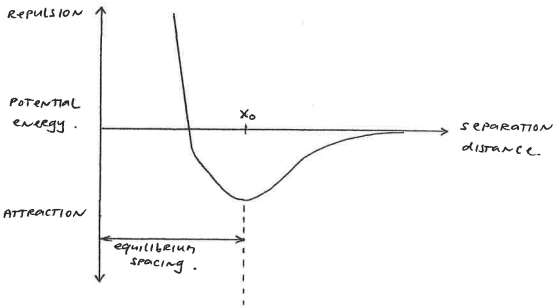
\includegraphics[width=0.8\linewidth]{exam./2019_atom_energy_sep.PNG}
        \caption{caption}
        %\label{fig:label}
    \end{figure}
    Where $x_0$ is the equilibrium spacing between two atoms.


    The force-separation relationship is as follows:
    \begin{figure}[htb]
        \centering
        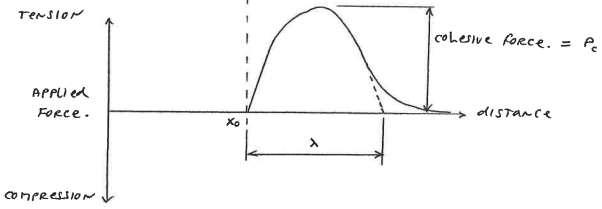
\includegraphics[width=0.8\linewidth]{exam./2019_atom-force-sep}
        \caption{caption}
        %\label{fig:label}
    \end{figure}
    Approximate the force-separation curve as half the period, $\lambda$, of a sine wave. Take origin at $x=x_0$, then we have:
    \begin{align}
        P&=P_c \sin^2\left(\frac{\pi x}{\lambda}\right)\\%\label{eq:label}
    \intertext{For small displacements, $\sin x \approx x$}
        \Rightarrow P&\simeq P_c \left(\frac{\pi x}{\lambda}\right)%\label{eq:label}
    \end{align}
    The bond stiffness is the slope of the force-displacement diagram
    \begin{equation}
        k = \frac Px = \frac{P_c \pi}{\lambda}%\label{eq:label}
    \end{equation}
    Relating this to the bulk properties of the material:
    \begin{equation}
        E = \frac{\sigma}{\varepsilon}\text{,}\;\;\;\; \sigma = \frac FA\text{,}\;\;\;\; \varepsilon=\frac{\text{displacement}}{\text{gauge length}}=\frac{x}{x_0}%\label{eq:label}
    \end{equation}
    




    \item fdsfa 
\end{enumerate}





\end{document}